\documentclass[usenames,dvipsnames]{beamer}
\usepackage{../../shared/styles/custom}
\usepackage{../../shared/styles/conventions}
\usepackage{tikz}
\usepackage{pdfpages}
\usetikzlibrary{arrows.meta, positioning, decorations.pathreplacing, calc, shadows}

% Pop quiz counter already defined in custom style

\newcommand{\E}{\mathbb{E}}

\title{Gradient Descent: The Foundation of Machine Learning Optimization}
\subtitle{From Taylor Series to Modern Deep Learning}
\date{\today}
\author{Nipun Batra and the teaching staff}
\institute{IIT Gandhinagar}

\begin{document}
  \maketitle

  \begin{frame}{Table of Contents}
    \tableofcontents
  \end{frame}

  \section{Mathematical Foundations}
  
  \begin{frame}{The Big Picture: Why Optimization Matters}
    \begin{keypointsbox}{}
    {\small \textbf{Core ML Problem:} Find best parameters $\vtheta^*$ for our model}
    \end{keypointsbox}
    
    \pause
    \textbf{Examples everywhere:}
    \begin{itemize}[<+->]
        \item Linear regression: Minimize $(y - \mX\vtheta)^2$
        \item Neural networks: Minimize classification/regression loss
        \item Logistic regression: Minimize cross-entropy loss
    \end{itemize}
    
    \pause
    \begin{alertbox}{The Challenge}
    {\small Most ML problems have \textbf{no closed-form solution!}}
    \end{alertbox}
  \end{frame}

  \begin{frame}{Gradient Intuition: Climbing Mountains}
    \textbf{Imagine you're hiking in dense fog and want to reach the valley:}
    
    \begin{itemize}[<+->]
        \item You can only feel the slope beneath your feet
        \item \textbf{Strategy:} Always step in the steepest downhill direction
        \item \textbf{Gradient} = Direction of steepest \textcolor{red}{uphill} (ascent)
        \item \textbf{Negative gradient} = Direction of steepest \textcolor{blue}{downhill} (descent)
    \end{itemize}
    
    \pause
    \begin{keypointsbox}{}
    \textbf{Key insight:} Gradient points in direction of steepest \textcolor{red}{ascent}
    
    So $-\nabla f$ points in direction of steepest \textcolor{blue}{descent}!
    \end{keypointsbox}
  \end{frame}

  \begin{frame}{Geometric Intuition with Level Sets}
    \begin{center}
    \includegraphics[scale=0.8]{../../maths/assets/mathematical-ml/figures/contour-x_squared_plus_y_squared_quiver-with-gradient.pdf}
    \end{center}
    
    \pause
    \textbf{Mathematical definition:} $\nabla f(x, y) = \begin{bmatrix} \frac{\partial f}{\partial x} \\ \frac{\partial f}{\partial y} \end{bmatrix}$
  \end{frame}

  \section{Taylor Series: The Mathematical Foundation}

  \begin{frame}{Why Taylor Series? The Key Insight}
    \begin{examplebox}{The Core Idea}
    {\small If we can't solve $\min f(\vx)$ exactly, let's approximate $f(\vx)$ locally!}
    \end{examplebox}
    
    \pause
    \textbf{Strategy:}
    \begin{itemize}[<+->]
        \item Replace complicated function with simpler approximation
        \item Optimize the approximation instead
        \item Move to new point and repeat
    \end{itemize}
    
    \pause
    \begin{alertbox}{Taylor Series Power}
    Any smooth function can be approximated by polynomials!
    \end{alertbox}
  \end{frame}

  \subsection{Univariate Taylor Series}

  \begin{frame}{Taylor Series: Starting with 1D}
    \textbf{Taylor series expansion around point $x_0$:}
    \begin{align}
        f(x) &= f(x_0) + f^{\prime}(x_0)(x-x_0) + \frac{1}{2}f^{\prime\prime}(x_0)(x-x_0)^2 + \frac{1}{6}f^{\prime\prime\prime}(x_0)(x-x_0)^3 + \ldots
    \end{align}
    
    \pause
    \textbf{Different orders of approximation:}
    \begin{itemize}[<+->]
        \item \textbf{Zero-order:} $f(x) \approx f(x_0)$ (constant)
        \item \textbf{First-order:} $f(x) \approx f(x_0) + f^{\prime}(x_0)(x-x_0)$ (linear)
        \item \textbf{Second-order:} adds $\frac{1}{2}f^{\prime\prime}(x_0)(x-x_0)^2$ (quadratic)
    \end{itemize}
  \end{frame}

  \begin{frame}{Visual: Tangent Line Approximation}
    \textbf{Linear approximation:} Use tangent line to approximate function locally

    \begin{center}
    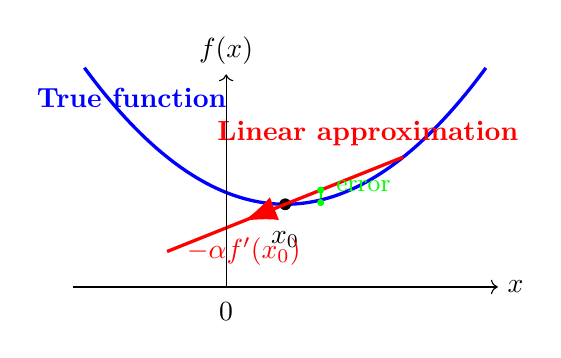
\begin{tikzpicture}[scale=1.5]
      % Original function (blue curve) - slightly steeper parabola
      \draw[blue, very thick, domain=-1.2:2.2, samples=100] 
        plot (\x, {0.4*(\x-0.5)*(\x-0.5) + 1.2});

      % Point of tangency
      \fill[black] (0.5,1.2) circle (0.05);
      \node[below] at (0.5,1.05) {$x_0$};

      % Tangent line (red) - extends further and clearer slope
      \draw[red, very thick, domain=-0.5:1.5] 
        plot (\x, {0.4*(\x-0.5) + 1.2});

      % Show the step we would take
      \draw[-{Latex[scale=1.8]}, red, thick] (0.5,1.2) -- (0.15,1.06);
      \node[red, below] at (0.15,1.0) {$-\alpha f^{\prime}(x_0)$};

      % Show approximation quality at different points
      \fill[green] (0.8, {0.4*(0.8-0.5)*0.4*(0.8-0.5) + 1.2}) circle (0.03);
      \fill[green] (0.8, {0.4*(0.8-0.5) + 1.2}) circle (0.03);
      \draw[green, dashed, thick] (0.8, {0.4*(0.8-0.5) + 1.2}) -- (0.8, {0.4*(0.8-0.5)*0.4*(0.8-0.5) + 1.2});
      \node[green, right] at (0.85,1.35) {\small error};

      % Labels
      \node[blue] at (-0.8,2.1) {\textbf{True function}};
      \node[red] at (1.2,1.8) {\textbf{Linear approximation}};

      % Axes with better spacing
      \draw[->] (-1.3,0.5) -- (2.3,0.5) node[right] {$x$};
      \draw[->] (0,0.5) -- (0,2.3) node[above] {$f(x)$};

      % Mark the zero point
      \node[below] at (0,0.45) {0};
    \end{tikzpicture}
    \end{center}

    \textbf{Key insight:} Tangent gives best local linear approximation!
  \end{frame}

  \begin{frame}{Adding Quadratic Term}
    \begin{center}
    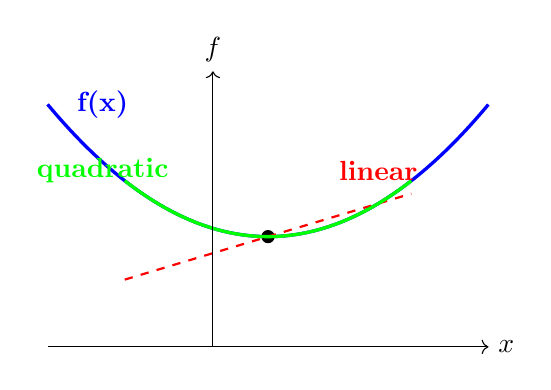
\begin{tikzpicture}[scale=1.4]
      % Original function (blue curve)
      \draw[blue, very thick, domain=-1.5:2.5, samples=100] 
        plot (\x, {0.3*(\x-0.5)*(\x-0.5) + 1});

      % Point of tangency
      \fill[black] (0.5,1) circle (0.06);

      % Tangent line (red, dashed)
      \draw[red, thick, dashed, domain=-0.8:1.8] 
        plot (\x, {0.3*(\x-0.5) + 1});

      % Quadratic approximation (green)
      \draw[green, very thick, domain=-0.8:1.8, samples=50] 
        plot (\x, {0.3*(\x-0.5)*(\x-0.5) + 1});

      % Labels
      \node[blue] at (-1,2.2) {\textbf{f(x)}};
      \node[red] at (1.5,1.6) {\textbf{linear}};
      \node[green] at (-1,1.6) {\textbf{quadratic}};

      % Axes
      \draw[->] (-1.5,0) -- (2.5,0) node[right] {$x$};
      \draw[->] (0,0) -- (0,2.5) node[above] {$f$};
    \end{tikzpicture}
    \end{center}

    \begin{keypointsbox}{}
    Higher-order = better approximation, but 1st-order is often sufficient!
    \end{keypointsbox}
  \end{frame}

  \begin{frame}{Concrete Example: $f(x) = \cos(x)$ at $x_0 = 0$}
    \textbf{Let's compute the derivatives:}
    \begin{itemize}[<+->]
        \item $f(0) = \cos(0) = 1$
        \item $f^{\prime}(0) = -\sin(0) = 0$
        \item $f^{\prime\prime}(0) = -\cos(0) = -1$
        \item $f^{\prime\prime\prime}(0) = \sin(0) = 0$
        \item $f^{(4)}(0) = \cos(0) = 1$
    \end{itemize}
    
    \pause
    \textbf{Taylor approximations:}
    \begin{align}
        \text{0th order:} \quad &f(x) \approx 1\\
        \text{2nd order:} \quad &f(x) \approx 1 - \frac{x^2}{2}\\
        \text{4th order:} \quad &f(x) \approx 1 - \frac{x^2}{2} + \frac{x^4}{24}
    \end{align}
  \end{frame}

  \subsection{Multivariate Taylor Series}

  \begin{frame}{Extension to Multiple Variables}
    \textbf{For function $f(\vx)$ around point $\vx_0$:}
    \begin{align}
        f(\vx) &= f(\vx_0) + \nabla f(\vx_0)^T(\vx-\vx_0) + \frac{1}{2}(\vx-\vx_0)^T\nabla^2 f(\vx_0)(\vx-\vx_0) + \ldots
    \end{align}
    
    \pause
    \textbf{Where:}
    \begin{itemize}[<+->]
        \item $\nabla f(\vx_0)$ is the \textbf{gradient} (vector of partial derivatives)
        \item $\nabla^2 f(\vx_0)$ is the \textbf{Hessian} (matrix of second derivatives)
        \item $(\vx-\vx_0) = \Delta\vx$ is the step vector
    \end{itemize}
  \end{frame}

  \begin{frame}{Understanding the Linear Term}
    \textbf{The first-order term:} $\nabla f(\vx_0)^T \Delta\vx$ where $\Delta\vx = \vx - \vx_0$
    
    \pause
    \textbf{For 2D case:} $\Delta\vx = \begin{bmatrix} \Delta x_1 \\ \Delta x_2 \end{bmatrix} = \begin{bmatrix} x_1 - x_{0,1} \\ x_2 - x_{0,2} \end{bmatrix}$
    
    \begin{center}
    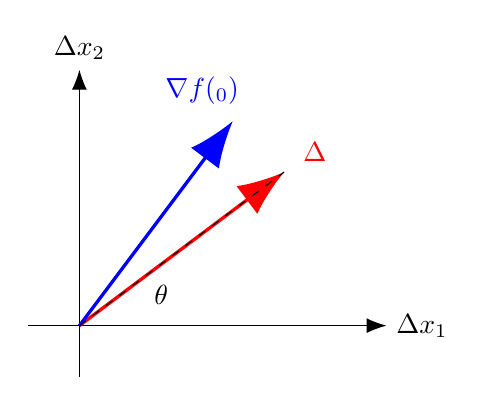
\begin{tikzpicture}[scale=1.3]
      % Draw coordinate system
      \draw[-{Latex[scale=1.5]}] (-0.5,0) -- (3,0) node[right] {$\Delta x_1$};
      \draw[-{Latex[scale=1.5]}] (0,-0.5) -- (0,2.5) node[above] {$\Delta x_2$};

      % Draw delta x vector
      \draw[-{Latex[scale=2]}, red, very thick] (0,0) -- (2,1.5);
      \node[red] at (2.3,1.7) {$\Delta\vx$};

      % Draw gradient vector
      \draw[-{Latex[scale=2]}, blue, very thick] (0,0) -- (1.5,2);
      \node[blue] at (1.2,2.3) {$\nabla f(\vx_0)$};

      % Show dot product angle
      \draw[dashed] (0,0) -- (1.33,1) -- (2,1.5);
      \node at (0.8,0.3) {$\theta$};
    \end{tikzpicture}
    \end{center}

    \textbf{Geometric interpretation:} $\nabla f(\vx_0)^T \Delta\vx = |\nabla f||\Delta\vx|\cos\theta$
  \end{frame}

  \begin{frame}{Visual: Multivariate Case with Level Sets}
    \begin{center}
    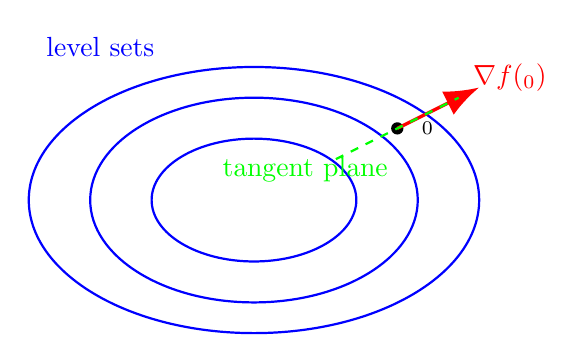
\begin{tikzpicture}[scale=1.3]
      % Level sets
      \draw[blue, thick] (0,0) ellipse (2.2 and 1.3);
      \draw[blue, thick] (0,0) ellipse (1.6 and 1);
      \draw[blue, thick] (0,0) ellipse (1 and 0.6);

      % Point x0
      \fill[black] (1.4,0.7) circle (0.06);
      \node at (1.7,0.7) {$\vx_0$};

      % Gradient vector (red)
      \draw[-{Latex[scale=1.5]}, red, very thick] (1.4,0.7) -- (2.2,1.1);
      \node[red] at (2.5,1.2) {$\nabla f(\vx_0)$};

      % Tangent plane indication
      \draw[green, thick, dashed] (0.8,0.4) -- (2.0,1.0);
      \node[green] at (0.5,0.3) {tangent plane};

      \node[blue] at (-1.5,1.5) {level sets};
    \end{tikzpicture}
    \end{center}

    \begin{keypointsbox}{}
    Gradient $\perp$ level sets, tangent plane $\perp$ gradient
    \end{keypointsbox}
  \end{frame}

  \begin{frame}{Why is Gradient Perpendicular to Level Sets?}
    \textbf{Mathematical insight:} Level set = \{$\vx : f(\vx) = c$\} for constant $c$

    \pause
    \textbf{On level sets:} Moving along the level curve keeps $f(\vx)$ constant
    \begin{itemize}
    \item If $\vx(t)$ parameterizes level curve: $f(\vx(t)) = c$ (constant)
    \item Taking derivative: $\frac{d}{dt}f(\vx(t)) = \nabla f(\vx) \cdot \vx'(t) = 0$
    \end{itemize}

    \pause
    \textbf{Conclusion:} $\nabla f(\vx) \perp \vx'(t)$ for any tangent direction $\vx'(t)$

    \pause
    \begin{center}
    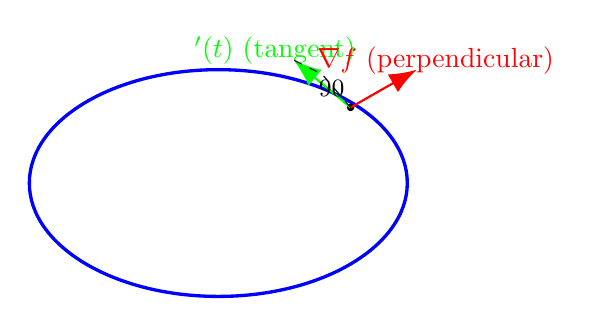
\begin{tikzpicture}[scale=1.2]
    % Level curve
    \draw[blue, very thick] (0,0) ellipse (2 and 1.2);
    % Point on curve
    \fill[black] (1.4,0.8) circle (0.04);
    % Tangent vector to level curve
    \draw[-{Latex[scale=1.5]}, green, thick] (1.4,0.8) -- (0.8,1.3);
    \node[green] at (0.6,1.4) {$\vx'(t)$ (tangent)};
    % Gradient vector (perpendicular)
    \draw[-{Latex[scale=1.5]}, red, thick] (1.4,0.8) -- (2.1,1.2);
    \node[red] at (2.3,1.3) {$\nabla f$ (perpendicular)};
    % Show perpendicular angle
    \draw[dashed] (1.4,0.8) -- (1.1,1.15) -- (0.8,1.3);
    \node at (1.2,1.0) {\small $90°$};
    \end{tikzpicture}
    \end{center}
  \end{frame}

  \section{From Taylor Series to Gradient Descent}

  \begin{frame}{The Key Question}
    \textbf{Goal:} Find $\Delta \vx$ such that $f(\vx_0 + \Delta \vx) < f(\vx_0)$
    
    \pause
    \textbf{Using first-order Taylor approximation:}
    \begin{align}
        f(\vx_0 + \Delta \vx) &\approx f(\vx_0) + \nabla f(\vx_0)^T \Delta \vx
    \end{align}
    
    \pause
    \textbf{For the function to decrease:}
    $$\nabla f(\vx_0)^T \Delta \vx < 0$$
    
    \pause
    \begin{alertbox}{Vector Geometry Reminder}
    For vectors $\mathbf{a}, \mathbf{b}$: $\mathbf{a}^T\mathbf{b} = |\mathbf{a}||\mathbf{b}|\cos(\theta)$
    
    \textbf{Most negative when:} $\cos(\theta) = -1$ (opposite directions!)
    \end{alertbox}
  \end{frame}

  \begin{frame}{Visual Derivation: Finding the Best Direction}
    \begin{center}
    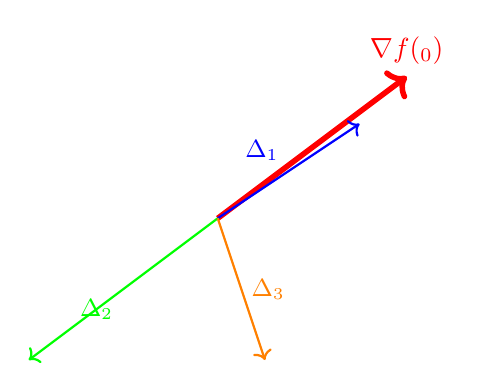
\begin{tikzpicture}[scale=1.2]
      % Draw gradient vector
      \draw[->, thick, red, line width=2pt] (0,0) -- (2,1.5) 
        node[above] {$\nabla f(\vx_0)$};
      
      % Draw potential step directions
      \draw[->, thick, blue] (0,0) -- (1.5,1) 
        node[midway, above left] {\small $\Delta \vx_1$};
      \draw[->, thick, green] (0,0) -- (-2,-1.5) 
        node[midway, below left] {\small $\Delta \vx_2$};
      \draw[->, thick, orange] (0,0) -- (0.5,-1.5) 
        node[midway, right] {\small $\Delta \vx_3$};
    \end{tikzpicture}
    \end{center}
    
    \pause
    \textbf{Dot products tell us the direction:}
    \begin{itemize}
        \item $\nabla f(\vx_0)^T \Delta \vx_1 > 0$ \textcolor{blue}{(increases function)}
        \item $\nabla f(\vx_0)^T \Delta \vx_2 < 0$ \textcolor{green}{(decreases function - good!)}
        \item $\nabla f(\vx_0)^T \Delta \vx_3 < 0$ \textcolor{orange}{(decreases function)}
    \end{itemize}
    
  \end{frame}

  \begin{frame}{The Optimal Choice: Direction of Steepest Descent}
    \begin{definitionbox}{Optimal Choice}
    $$\Delta \vx = -\alpha \nabla f(\vx_0), \quad \alpha > 0$$
    \end{definitionbox}
    
    \pause
    \textbf{Why this choice?}
    \begin{itemize}[<+->]
        \item $-\nabla f(\vx_0)$ points in direction of steepest descent
        \item $\alpha > 0$ controls the step size
        \item Guarantees $\nabla f(\vx_0)^T \Delta\vx < 0$ (function decrease)
    \end{itemize}
    
    \pause
    \begin{keypointsbox}{}
    This gives us the fundamental gradient descent step!
    \end{keypointsbox}
  \end{frame}

  \begin{frame}{The Gradient Descent Update Rule}
    \textbf{This gives us the gradient descent update:}
    $$\vx_{\text{new}} = \vx_{\text{old}} - \alpha \nabla f(\vx_{\text{old}})$$
    
    \pause
    \begin{definitionbox}{Gradient Descent Algorithm}
    An iterative first-order optimization method for finding local minima
    \end{definitionbox}
    
    \pause
    \textbf{Key properties:}
    \begin{itemize}[<+->]
        \item Uses only first derivatives (gradients)
        \item Greedy local search
        \item Guaranteed convergence for convex functions
        \item Foundation of modern machine learning
    \end{itemize}
  \end{frame}

  \stepcounter{popquiz}
  \begin{frame}{Pop Quiz \#\thepopquiz: Understanding the Derivation}
    \begin{popquizbox}{\thepopquiz}
    Consider $f(x) = x^2 + 2$ at point $x_0 = 2$.
    
    \textbf{Questions:}
    \begin{enumerate}
        \item What is $f(x_0)$ and $f^{\prime}(x_0)$?
        \item Write the 1st-order Taylor approximation
        \item If we take step $\Delta x = -0.1 \cdot f^{\prime}(x_0)$, what is our new $x$?
        \item Will the function value decrease?
    \end{enumerate}
    \end{popquizbox}
  \end{frame}

  \section{The Gradient Descent Algorithm}

  \begin{frame}{The Complete Algorithm}
    \textbf{Algorithm Steps:}
    \begin{enumerate}[<+->]
        \item \textbf{Initialize:} Choose starting point $\vtheta_0$
        \item \textbf{Repeat until convergence:}
        \begin{itemize}
            \item Compute gradient: $\vg_t = \nabla f(\vtheta_t)$
            \item Update parameters: $\vtheta_{t+1} = \vtheta_t - \alpha \vg_t$  
            \item Check stopping criterion
        \end{itemize}
    \end{enumerate}
    
    \pause
    \textbf{Key hyperparameter: Learning rate $\alpha$}
    
    \pause
    \begin{keypointsbox}{}
    Learning rate selection is crucial for success!
    \end{keypointsbox}
  \end{frame}

  \begin{frame}{Animated Gradient Descent in Action}
    \textbf{Watch how gradient descent finds the minimum:}
    
    \begin{center}
    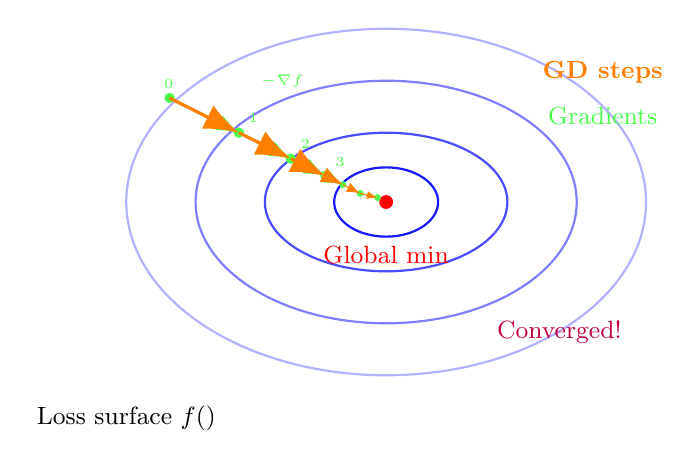
\begin{tikzpicture}[scale=1.1]
      % Draw loss surface contours
      \draw[blue!30, thick] (0,0) ellipse (3 and 2);
      \draw[blue!50, thick] (0,0) ellipse (2.2 and 1.4);
      \draw[blue!70, thick] (0,0) ellipse (1.4 and 0.8);
      \draw[blue!90, thick] (0,0) ellipse (0.6 and 0.4);
      
      % Global minimum
      \fill[red] (0,0) circle (0.08);
      \node[red, below] at (0,-0.4) {\small Global min};
      
      % Animated gradient descent path
      \onslide<2->{
        % Step 1: Start point
        \coordinate (p0) at (-2.5, 1.2);
        \fill[green!70] (p0) circle (0.06);
        \node[green!70, above] at (p0) {\tiny $\vtheta_0$};
        
        % Draw gradient arrow at start
        \draw[-{Latex[scale=1.2]}, green!70, thick] (p0) -- ++(0.8, -0.4);
        \node[green!70] at (-1.2, 1.4) {\tiny $-\nabla f$};
      }
      
      \onslide<3->{
        % Step 2
        \coordinate (p1) at (-1.7, 0.8);
        \fill[green!70] (p1) circle (0.06);
        \node[green!70, above right] at (p1) {\tiny $\vtheta_1$};
        \draw[-{Latex[scale=1.5]}, orange, very thick] (p0) -- (p1);
        
        % Gradient at step 2
        \draw[-{Latex[scale=1.2]}, green!70, thick] (p1) -- ++(0.6, -0.3);
      }
      
      \onslide<4->{
        % Step 3
        \coordinate (p2) at (-1.1, 0.5);
        \fill[green!70] (p2) circle (0.06);
        \node[green!70, above right] at (p2) {\tiny $\vtheta_2$};
        \draw[-{Latex[scale=1.5]}, orange, very thick] (p1) -- (p2);
        
        % Gradient at step 3
        \draw[-{Latex[scale=1.2]}, green!70, thick] (p2) -- ++(0.4, -0.2);
      }
      
      \onslide<5->{
        % Step 4
        \coordinate (p3) at (-0.7, 0.3);
        \fill[green!70] (p3) circle (0.06);
        \node[green!70, above right] at (p3) {\tiny $\vtheta_3$};
        \draw[-{Latex[scale=1.5]}, orange, very thick] (p2) -- (p3);
        
        % Gradient getting smaller
        \draw[-{Latex[scale=1.0]}, green!70, thick] (p3) -- ++(0.2, -0.1);
      }
      
      \onslide<6->{
        % Final steps to convergence
        \coordinate (p4) at (-0.5, 0.2);
        \coordinate (p5) at (-0.3, 0.1);
        \coordinate (p6) at (-0.1, 0.05);
        
        \foreach \p in {p4, p5, p6} {
          \fill[green!70] (\p) circle (0.04);
        }
        \draw[-{Latex[scale=1.2]}, orange, thick] (p3) -- (p4);
        \draw[-{Latex[scale=1.0]}, orange] (p4) -- (p5);
        \draw[-{Latex[scale=0.8]}, orange] (p5) -- (p6);
        
        % Show convergence
        \node[purple, font=\small] at (2, -1.5) {Converged!};
      }
      
      % Labels
      \node at (-3, -2.5) {\small Loss surface $f(\vtheta)$};
      \onslide<2->{\node[orange] at (2.5, 1.5) {\small \textbf{GD steps}};}
      \onslide<3->{\node[green!70] at (2.5, 1.0) {\small Gradients};}
    \end{tikzpicture}
    \end{center}
    
    \vspace{0.3cm}
    \onslide<7>{
    \begin{theorembox}{Key Insight}
    {\small Steps get \textbf{smaller} as we approach the minimum because $|\nabla f| \to 0$!}
    \end{theorembox}
    }
  \end{frame}

  \begin{frame}{Learning Rate: The Step Size}
    \textbf{The learning rate $\alpha$ controls how big steps we take:}
    
    \begin{itemize}[<+->]
        \item \textbf{Too small $\alpha$:} Slow convergence
        \item \textbf{Good $\alpha$:} Fast, stable convergence  
        \item \textbf{Too large $\alpha$:} Overshooting, instability
        \item \textbf{Way too large $\alpha$:} Divergence!
    \end{itemize}
    
    \pause
    \begin{center}
    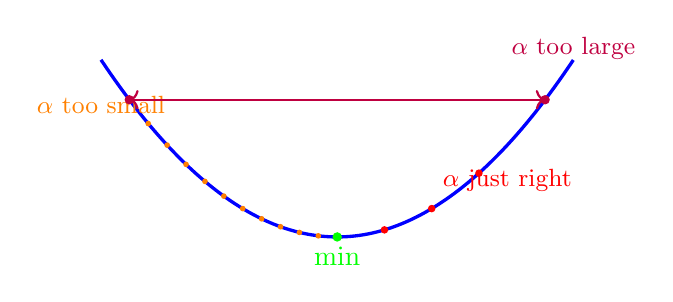
\begin{tikzpicture}[scale=1.2]
      % Quadratic function
      \draw[blue, very thick, domain=-2.5:2.5, samples=100] 
        plot (\x, {0.3*\x*\x + 0.2});

      % Minimum
      \fill[green] (0,0.2) circle (0.05);
      \node[green] at (0,0) {min};

      % Small alpha (many small steps)
      \foreach \x in {-2,-1.8,-1.6,-1.4,-1.2,-1,-0.8,-0.6,-0.4,-0.2} {
        \fill[orange] (\x, {0.3*\x*\x + 0.2}) circle (0.03);
      }
      \node[orange] at (-2.5,1.6) {\small $\alpha$ too small};

      % Good alpha (reasonable steps)  
      \foreach \x in {1.5,1,0.5} {
        \fill[red] (\x, {0.3*\x*\x + 0.2}) circle (0.04);
      }
      \node[red] at (1.8,0.8) {\small $\alpha$ just right};

      % Large alpha (overshoot)
      \fill[purple] (2.2, {0.3*2.2*2.2 + 0.2}) circle (0.05);
      \fill[purple] (-2.2, {0.3*2.2*2.2 + 0.2}) circle (0.05);
      \draw[purple, thick, <->] (2.2, {0.3*2.2*2.2 + 0.2}) -- (-2.2, {0.3*2.2*2.2 + 0.2});
      \node[purple] at (2.5,2.2) {\small $\alpha$ too large};
    \end{tikzpicture}
    \end{center}
  \end{frame}

  \begin{frame}{Learning Rate Visualization: Too Small}
    \textbf{$\alpha = 0.01$: Convergence is slow but stable}
    \begin{center}
    \includegraphics[scale=0.8]{../../maths/assets/mathematical-ml/figures/gd-lr-0.01.pdf}
    \end{center}
    
    \begin{alertbox}{Problem}
    Takes many iterations to reach the minimum. Computationally expensive!
    \end{alertbox}
  \end{frame}

  \begin{frame}{Learning Rate: Just Right}
    \textbf{$\alpha = 0.1$: Good balance: Fast and stable convergence}
    \begin{center}
    \includegraphics[scale=0.8]{../../maths/assets/mathematical-ml/figures/gd-lr-0.1.pdf}
    \end{center}
    
    \begin{keypointsbox}{}
    Perfect balance: Fast convergence + Stability
    \end{keypointsbox}
  \end{frame}

  \begin{frame}{Learning Rate: Too Large}
    \textbf{$\alpha = 0.8$: Fast but may overshoot}
    \begin{center}
    \includegraphics[scale=0.8]{../../maths/assets/mathematical-ml/figures/gd-lr-0.8.pdf}
    \end{center}
    
    \begin{alertbox}{Warning}
    Quick convergence but risk of instability. Watch out for oscillations!
    \end{alertbox}
  \end{frame}

  \begin{frame}{Learning Rate: Disaster}
    \textbf{$\alpha = 1.01$: Divergence! Function values explode}
    \begin{center}
    \includegraphics[scale=0.8]{../../maths/assets/mathematical-ml/figures/gd-lr-1.01.pdf}
    \end{center}
    
    \begin{alertbox}{Disaster Zone}
    The algorithm diverges. Always monitor your loss curves!
    \end{alertbox}
  \end{frame}

  \begin{frame}{Learning Rate Showdown: All Together}
    \textbf{Compare different learning rates side by side:}
    
    \begin{center}
    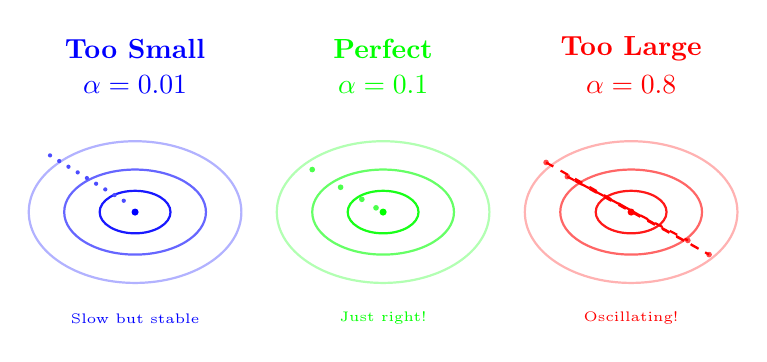
\begin{tikzpicture}[scale=0.9]
      % Left: Too small learning rate
      \begin{scope}[shift={(-3.5,0)}]
        \draw[blue!30, thick] (0,0) ellipse (1.5 and 1);
        \draw[blue!60, thick] (0,0) ellipse (1.0 and 0.6);
        \draw[blue!90, thick] (0,0) ellipse (0.5 and 0.3);
        \fill[blue] (0,0) circle (0.05);
        \node[blue, font=\small, font=\bfseries] at (0, 1.8) {$\alpha = 0.01$};
        
        % Many small steps
        \foreach \step in {0,...,8} {
          \pgfmathparse{-1.2 + \step * 0.13}
          \let\x\pgfmathresult
          \pgfmathparse{0.8 - \step * 0.08}
          \let\y\pgfmathresult
          \fill[blue!70] (\x, \y) circle (0.03);
        }
        \node[blue] at (0, -1.5) {\tiny Slow but stable};
      \end{scope}
      
      % Center: Perfect learning rate
      \begin{scope}[shift={(0,0)}]
        \draw[green!30, thick] (0,0) ellipse (1.5 and 1);
        \draw[green!60, thick] (0,0) ellipse (1.0 and 0.6);
        \draw[green!90, thick] (0,0) ellipse (0.5 and 0.3);
        \fill[green] (0,0) circle (0.05);
        \node[green, font=\small, font=\bfseries] at (0, 1.8) {$\alpha = 0.1$};
        
        % Perfect steps
        \foreach \step/\x/\y in {0/-1.0/0.6, 1/-0.6/0.35, 2/-0.3/0.18, 3/-0.1/0.06} {
          \fill[green!70] (\x, \y) circle (0.04);
        }
        \node[green] at (0, -1.5) {\tiny Just right!};
      \end{scope}
      
      % Right: Too large learning rate
      \begin{scope}[shift={(3.5,0)}]
        \draw[red!30, thick] (0,0) ellipse (1.5 and 1);
        \draw[red!60, thick] (0,0) ellipse (1.0 and 0.6);
        \draw[red!90, thick] (0,0) ellipse (0.5 and 0.3);
        \fill[red] (0,0) circle (0.05);
        \node[red, font=\small, font=\bfseries] at (0, 1.8) {$\alpha = 0.8$};
        
        % Oscillating behavior
        \fill[red!70] (-1.2, 0.7) circle (0.04);
        \fill[red!70] (1.1, -0.6) circle (0.04);
        \fill[red!70] (-0.9, 0.5) circle (0.04);
        \fill[red!70] (0.8, -0.4) circle (0.04);
        \draw[red, thick, dashed] (-1.2, 0.7) -- (1.1, -0.6) -- (-0.9, 0.5) -- (0.8, -0.4);
        \node[red] at (0, -1.5) {\tiny Oscillating!};
      \end{scope}
      
      % Labels
      \node at (-3.5, 2.3) {\textbf{\color{blue}Too Small}};
      \node at (0, 2.3) {\textbf{\color{green}Perfect}};
      \node at (3.5, 2.3) {\textbf{\color{red}Too Large}};
    \end{tikzpicture}
    \end{center}
    
    \vspace{0.5cm}
    \begin{theorembox}{Goldilocks Principle}
    {\small Not too small, not too large - learning rate must be \textbf{just right}!}
    \end{theorembox}
    
    \begin{keypointsbox}{}
    {\small \textbf{Pro tip:} Start with $\alpha \in [0.01, 0.1]$ and adjust based on loss curves}
    \end{keypointsbox}
  \end{frame}

  \section{Gradient Descent for Linear Regression}

  \begin{frame}{Linear Regression: Our First Application}
    \textbf{Problem:} Learn $y = \theta_0 + \theta_1 x$ from data
    
    \begin{center}
    \begin{tabular}{|c|c|}
        \hline
        \textbf{x} & \textbf{y} \\
        \hline
        1 & 1 \\
        2 & 2 \\
        3 & 3 \\
        \hline
    \end{tabular}
    \end{center}
    
    \pause
    \textbf{Cost Function (Mean Squared Error):}
    $$\MSE(\theta_0, \theta_1) = \frac{1}{n}\sum_{i=1}^n (y_i - \hat{y}_i)^2 = \frac{1}{n}\sum_{i=1}^n (y_i - \theta_0 - \theta_1 x_i)^2$$
    
    \pause
    \textbf{Goal:} $(\theta_0^*, \theta_1^*) = \argmin_{\theta_0, \theta_1} \MSE(\theta_0, \theta_1)$
  \end{frame}

  \begin{frame}{Computing Gradients for Linear Regression}
    \textbf{We need:} $\nabla \MSE = \begin{bmatrix} \frac{\partial \MSE}{\partial \theta_0} \\ \frac{\partial \MSE}{\partial \theta_1} \end{bmatrix}$
    
    \pause
    \textbf{Let's compute each partial derivative:}
    
    \begin{align}
        \frac{\partial \MSE}{\partial \theta_0} &= \frac{2}{n}\sum_{i=1}^n (y_i - \theta_0 - \theta_1 x_i)(-1)\\
        &= -\frac{2}{n}\sum_{i=1}^n \epsilon_i
    \end{align}
    
    \pause
    \begin{align}
        \frac{\partial \MSE}{\partial \theta_1} &= \frac{2}{n}\sum_{i=1}^n (y_i - \theta_0 - \theta_1 x_i)(-x_i)\\
        &= -\frac{2}{n}\sum_{i=1}^n \epsilon_i x_i
    \end{align}
    
    where $\epsilon_i = y_i - \hat{y}_i$ is the residual.
  \end{frame}

  \begin{frame}{Step-by-Step Example: Setup}
    \textbf{Initial values:} $\theta_0 = 4, \theta_1 = 0$, \textbf{Learning rate:} $\alpha = 0.1$
    
    \pause
    \textbf{Iteration 1 - Predictions:}
    \begin{itemize}[<+->]
        \item $\hat{y}_1 = \theta_0 + \theta_1 \cdot 1 = 4 + 0 \cdot 1 = 4$
        \item $\hat{y}_2 = \theta_0 + \theta_1 \cdot 2 = 4 + 0 \cdot 2 = 4$ 
        \item $\hat{y}_3 = \theta_0 + \theta_1 \cdot 3 = 4 + 0 \cdot 3 = 4$
    \end{itemize}
    
    \pause
    \textbf{Errors (residuals):}
    \begin{itemize}[<+->]
        \item $\epsilon_1 = y_1 - \hat{y}_1 = 1 - 4 = -3$
        \item $\epsilon_2 = y_2 - \hat{y}_2 = 2 - 4 = -2$
        \item $\epsilon_3 = y_3 - \hat{y}_3 = 3 - 4 = -1$
    \end{itemize}
  \end{frame}

  \begin{frame}{Step-by-Step Example: Gradients}
    \textbf{Compute gradients:}
    \begin{itemize}[<+->]
        \item $\frac{\partial \MSE}{\partial \theta_0} = -\frac{2}{3}(-3-2-1) = -\frac{2}{3}(-6) = 4$
        \item $\frac{\partial \MSE}{\partial \theta_1} = -\frac{2}{3}(-3 \cdot 1 - 2 \cdot 2 - 1 \cdot 3) = -\frac{2}{3}(-10) = 6.67$
    \end{itemize}
    
    \pause
    \textbf{Parameter updates:}
    \begin{itemize}[<+->]
        \item $\theta_0 = 4 - 0.1 \times 4 = 3.6$
        \item $\theta_1 = 0 - 0.1 \times 6.67 = -0.67$
    \end{itemize}
    
    \pause
    \begin{keypointsbox}{}
    New parameters: $(\theta_0, \theta_1) = (3.6, -0.67)$
    
    We moved closer to the true solution $(0, 1)$!
    \end{keypointsbox}
  \end{frame}

  \begin{frame}{Visual Journey: Gradient Descent in Action}
    \begin{center}
    \begin{tikzpicture}[scale=1.1]
      % Loss contours (elliptical)
      \draw[blue, thick] (0,0) ellipse (3.5 and 2);
      \draw[blue, thick] (0,0) ellipse (2.5 and 1.4);
      \draw[blue, thick] (0,0) ellipse (1.8 and 1);
      \draw[blue, thick] (0,0) ellipse (1.1 and 0.6);
      \draw[blue, thick] (0,0) ellipse (0.6 and 0.35);

      % Minimum
      \fill[green] (0,0) circle (0.06);
      \node[green, below] at (0,-0.3) {\small $\vtheta^*$};

      % GD path (step by step with overlays)
      \only<1>{
        \coordinate (p1) at (3,1.5);
        \fill[red] (p1) circle (0.08);
        \node[red] at (3.3,1.7) {\small $\vtheta_0$};
      }
      
      \only<2->{
        \coordinate (p1) at (3,1.5);
        \coordinate (p2) at (2.1,1);
        \fill[red] (p1) circle (0.06);
        \draw[-{Latex[scale=1.5]}, red, thick] (p1) -- (p2);
        \fill[red] (p2) circle (0.08);
        \node[red] at (2.3,1.3) {\small $\vtheta_1$};
      }
      
      \only<3->{
        \coordinate (p3) at (1.4,0.6);
        \draw[-{Latex[scale=1.5]}, red, thick] (p2) -- (p3);
        \fill[red] (p3) circle (0.08);
        \node[red] at (1.6,0.8) {\small $\vtheta_2$};
      }
      
      \only<4->{
        \coordinate (p4) at (0.8,0.3);
        \draw[-{Latex[scale=1.5]}, red, thick] (p3) -- (p4);
        \fill[red] (p4) circle (0.08);
        \node[red] at (1,0.5) {\small $\vtheta_3$};
      }
      
      \only<5->{
        \coordinate (p5) at (0.4,0.15);
        \draw[-{Latex[scale=1.5]}, red, thick] (p4) -- (p5);
        \fill[red] (p5) circle (0.08);
        \node[red] at (0.6,0.3) {\small $\vtheta_4$};
      }
      
      \only<6->{
        \coordinate (p6) at (0.2,0.07);
        \draw[-{Latex[scale=1.5]}, red, thick] (p5) -- (p6);
        \fill[red] (p6) circle (0.08);
        \node[red] at (0.4,0.15) {\small $\vtheta_5$};
      }
      
      \only<7>{
        \coordinate (p7) at (0.05,0.02);
        \draw[-{Latex[scale=1.5]}, red, thick] (p6) -- (p7);
        \fill[red] (p7) circle (0.08);
        \node[red] at (0.2,0.08) {\small $\vtheta_6$};
      }

      \node[blue] at (-2.5,1.8) {\small loss contours};
    \end{tikzpicture}
    \end{center}
    
    \pause
    \begin{keypointsbox}{}
    {\small Steps get smaller as we approach minimum (gradient magnitude decreases)!}
    \end{keypointsbox}
  \end{frame}

  \section{Variants of Gradient Descent}

  \begin{frame}{The Gradient Descent Family}
    \textbf{Three main variants based on data usage:}
    
    \begin{definitionbox}{Batch Gradient Descent}
    Use \textcolor{red}{all} training data to compute each gradient
    \end{definitionbox}
    
    \begin{definitionbox}{Stochastic Gradient Descent (SGD)}
    Use \textcolor{red}{one} sample to compute each gradient
    \end{definitionbox}
    
    \begin{definitionbox}{Mini-batch Gradient Descent}
    Use a \textcolor{red}{small batch} of samples to compute each gradient
    \end{definitionbox}
  \end{frame}

  \begin{frame}{Comparison: Batch vs SGD vs Mini-batch}
    \begin{center}
    \begin{tabular}{|l|c|c|c|}
        \hline
        \textbf{Method} & \textbf{Data/update} & \textbf{Updates/epoch} & \textbf{Convergence} \\
        \hline
        Batch GD & $n$ (all) & 1 & Smooth \\
        \hline
        SGD & 1 & $n$ & Noisy \\
        \hline
        Mini-batch & $b$ & $n/b$ & Balanced \\
        \hline
    \end{tabular}
    \end{center}
    
    \pause
    \begin{keypointsbox}{}
    {\scriptsize \textbf{Standard:} Mini-batch GD (batches 32-256)
    \begin{itemize}
        \item Balance of stability and efficiency
        \item Parallel computation on GPUs
        \item Better estimates than pure SGD
    \end{itemize}}
    \end{keypointsbox}
  \end{frame}

  \begin{frame}{SGD: The Noisy Path}
    \textbf{SGD uses one sample at a time for updates}
    
    \begin{center}
    \includegraphics[scale=0.5]{../../maths/assets/mathematical-ml/figures/gradient-descent-3-functions.pdf}
    \end{center}
    
    \pause
    \textbf{Trade-offs:}
    \begin{itemize}[<+->]
        \item \textbf{Pro:} Fast updates, can escape local minima
        \item \textbf{Con:} Noisy convergence, may not reach exact minimum
        \item \textbf{Key insight:} Noise can be beneficial for non-convex problems!
    \end{itemize}
  \end{frame}

  \section{Mathematical Properties}

  \begin{frame}{Step 1: The Modern ML Computational Challenge}
    \textbf{Real-world machine learning problems:}
    
    \begin{itemize}[<+->]
        \item \textbf{Massive datasets:} $n = 1,000,000+$ examples (ImageNet, web data)
        \item \textbf{Large models:} Neural networks with millions of parameters
        \item \textbf{Complex computations:} Each forward pass through model is expensive
    \end{itemize}
    
    \pause
    \textbf{The gradient computation bottleneck:}
    $$\nabla L(\vtheta) = \nabla \left(\frac{1}{n}\sum_{i=1}^n \ell(f(\vx_i;\vtheta),y_i)\right)$$
    
    \pause
    \begin{alertbox}{The Problem}
    Computing $f(\vx_i;\vtheta)$ for ALL $n$ samples is too slow!
    
    Need: Fast approximation that still gives good direction
    \end{alertbox}
  \end{frame}

  \begin{frame}{Step 2: Computational Graph - Can We Break This?}
    \textbf{Current approach:} Sum first, then take gradient
    
    \begin{center}
    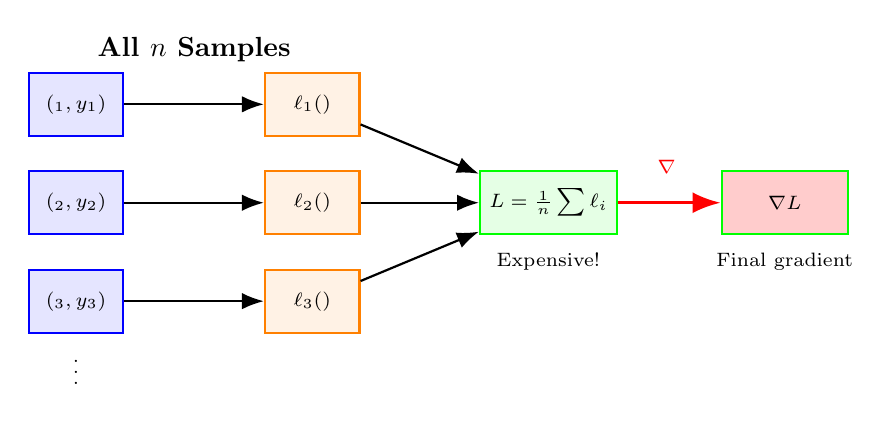
\begin{tikzpicture}[
        node distance=1.5cm,
        sample/.style={rectangle, draw=blue, fill=blue!10, thick, minimum width=1.2cm, minimum height=0.8cm},
        loss/.style={rectangle, draw=orange, fill=orange!10, thick, minimum width=1.2cm, minimum height=0.8cm},
        grad/.style={rectangle, draw=green, fill=green!10, thick, minimum width=1.6cm, minimum height=0.8cm},
        arrow/.style={-{Latex[scale=1.2]}, thick}
    ]

    % Individual samples
    \node[sample] (s1) at (0,2.5) {\scriptsize $(\vx_1,y_1)$};
    \node[sample] (s2) at (0,1.25) {\scriptsize $(\vx_2,y_2)$};
    \node[sample] (s3) at (0,0) {\scriptsize $(\vx_3,y_3)$};
    \node at (0,-0.8) {\scriptsize $\vdots$};

    % Individual losses  
    \node[loss] (l1) at (3,2.5) {\scriptsize $\ell_1(\vtheta)$};
    \node[loss] (l2) at (3,1.25) {\scriptsize $\ell_2(\vtheta)$};
    \node[loss] (l3) at (3,0) {\scriptsize $\ell_3(\vtheta)$};

    % Total loss
    \node[grad] (total) at (6,1.25) {\scriptsize $L = \frac{1}{n}\sum \ell_i$};

    % Final gradient
    \node[grad, fill=red!20] (final) at (9,1.25) {\scriptsize $\nabla L$};

    % Arrows
    \draw[arrow] (s1) -- (l1);
    \draw[arrow] (s2) -- (l2);
    \draw[arrow] (s3) -- (l3);
    \draw[arrow] (l1) -- (total);
    \draw[arrow] (l2) -- (total);
    \draw[arrow] (l3) -- (total);
    
    % Gradient operator arrow
    \draw[arrow, red, very thick] (total) -- (final);
    \node[red] at (7.5,1.7) {\scriptsize $\nabla$};

    % Labels
    \node at (1.5,3.2) {\textbf{All $n$ Samples}};
    \node at (6,0.5) {\scriptsize Expensive!};
    \node at (9,0.5) {\scriptsize Final gradient};
    \end{tikzpicture}
    \end{center}
    
    \begin{keypointsbox}{}
    {\scriptsize \textbf{Problem:} Computing losses for all $n$ samples is expensive!}
    \end{keypointsbox}
  \end{frame}

  \begin{frame}{Step 3: The Linearity Insight - What If We Flip the Order?}
    \begin{center}
    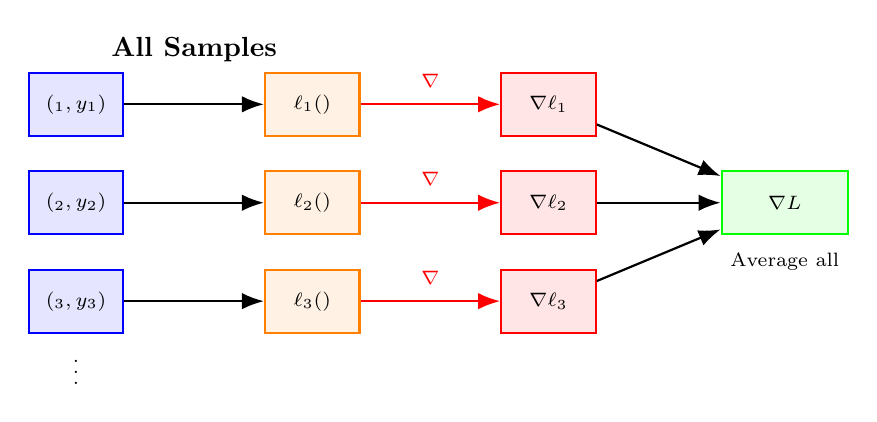
\begin{tikzpicture}[
        node distance=1.5cm,
        sample/.style={rectangle, draw=blue, fill=blue!10, thick, minimum width=1.2cm, minimum height=0.8cm},
        loss/.style={rectangle, draw=orange, fill=orange!10, thick, minimum width=1.2cm, minimum height=0.8cm},
        grad/.style={rectangle, draw=red, fill=red!10, thick, minimum width=1.2cm, minimum height=0.8cm},
        avg/.style={rectangle, draw=green, fill=green!10, thick, minimum width=1.6cm, minimum height=0.8cm},
        arrow/.style={-{Latex[scale=1.2]}, thick}
    ]

    % Individual samples
    \node[sample] (s1) at (0,2.5) {\scriptsize $(\vx_1,y_1)$};
    \node[sample] (s2) at (0,1.25) {\scriptsize $(\vx_2,y_2)$};
    \node[sample] (s3) at (0,0) {\scriptsize $(\vx_3,y_3)$};
    \node at (0,-0.8) {\scriptsize $\vdots$};

    % Individual losses  
    \node[loss] (l1) at (3,2.5) {\scriptsize $\ell_1(\vtheta)$};
    \node[loss] (l2) at (3,1.25) {\scriptsize $\ell_2(\vtheta)$};
    \node[loss] (l3) at (3,0) {\scriptsize $\ell_3(\vtheta)$};

    % Individual gradients
    \node[grad] (g1) at (6,2.5) {\scriptsize $\nabla\ell_1$};
    \node[grad] (g2) at (6,1.25) {\scriptsize $\nabla\ell_2$};
    \node[grad] (g3) at (6,0) {\scriptsize $\nabla\ell_3$};

    % True gradient (average)
    \node[avg] (gtrue) at (9,1.25) {\scriptsize $\nabla L$};

    % Arrows
    \draw[arrow] (s1) -- (l1);
    \draw[arrow] (s2) -- (l2);
    \draw[arrow] (s3) -- (l3);
    
    % Gradient operator arrows
    \draw[arrow, red, thick] (l1) -- (g1);
    \draw[arrow, red, thick] (l2) -- (g2);
    \draw[arrow, red, thick] (l3) -- (g3);
    \node[red] at (4.5,2.8) {\scriptsize $\nabla$};
    \node[red] at (4.5,1.55) {\scriptsize $\nabla$};
    \node[red] at (4.5,0.3) {\scriptsize $\nabla$};
    
    \draw[arrow] (g1) -- (gtrue);
    \draw[arrow] (g2) -- (gtrue);
    \draw[arrow] (g3) -- (gtrue);

    % Labels
    \node at (1.5,3.2) {\textbf{All Samples}};
    \node at (9,0.5) {\scriptsize Average all};
    \end{tikzpicture}
    \end{center}

    \begin{theorembox}{Linearity of Gradient}
    $\nabla L = \frac{1}{n}\sum_{i=1}^n \nabla \ell_i$
    \end{theorembox}
  \end{frame}

  \begin{frame}{Step 4: The Mathematical Equivalence - Linearity of Gradient}
    \textbf{Mathematical equivalence:}
    \begin{align}
    \nabla L(\vtheta) &= \nabla \left(\frac{1}{n}\sum_{i=1}^n \ell(f(\vx_i;\vtheta),y_i)\right)\\
    &= \frac{1}{n}\sum_{i=1}^n \nabla \ell(f(\vx_i;\vtheta),y_i)
    \end{align}

    \begin{keypointsbox}{}
    \textbf{This linearity property is the foundation for all gradient-based optimization!}
    \end{keypointsbox}
  \end{frame}

  \begin{frame}{Step 5: SGD as Unbiased Estimator - The Solution}
    {\small \textbf{SGD solution:} Sample one gradient instead of all $n$!}
    
    \pause
    {\small \textbf{Estimate:} $\nabla \tilde{L}(\vtheta) = \nabla \ell(f(\vx_j;\vtheta),y_j)$ for random $j$}

    \pause
    \begin{center}
    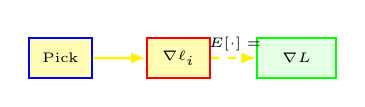
\begin{tikzpicture}[
        node distance=1cm,
        sample/.style={rectangle, draw=blue, fill=blue!10, thick, minimum width=0.8cm, minimum height=0.5cm},
        grad/.style={rectangle, draw=red, fill=red!10, thick, minimum width=0.8cm, minimum height=0.5cm},
        avg/.style={rectangle, draw=green, fill=green!10, thick, minimum width=1cm, minimum height=0.5cm},
        arrow/.style={-{Latex[scale=0.8]}, thick},
        scale=0.6
    ]

    % Show sampling process
    \node[sample, fill=yellow!30] (sgd) at (0,0.5) {\tiny Pick};
    \node[grad, fill=yellow!30] (gsgd) at (2.5,0.5) {\tiny $\nabla\ell_i$};
    
    % True gradient reference
    \node[avg] (gtrue) at (5,0.5) {\tiny $\nabla L$};

    % Arrows
    \draw[arrow, yellow, thick] (sgd) -- (gsgd);
    \draw[arrow, yellow, dashed] (gsgd) -- (gtrue);

    % Show expectation
    \node at (3.7,0.8) {\tiny $\E[\cdot] =$};
    \end{tikzpicture}
    \end{center}

    \begin{alertbox}{Unbiased Property}
    {\scriptsize $\E[\nabla \tilde{L}(\vtheta)] = \nabla L(\vtheta)$ - correct direction on average!}
    \end{alertbox}
  \end{frame}

  \begin{frame}{The Unbiased Property: Mathematical Proof}
    \begin{theorembox}{SGD Unbiased Estimator Property}
      {\small
    $$\E[\nabla \tilde{L}(\vtheta)] = \nabla L(\vtheta)$$
      }
    \end{theorembox}

    \pause
    {\small
    \begin{align}
    \E[\nabla \tilde{L}(\vtheta)] &= \E\left[\nabla \ell(f(\vx_j;\vtheta),y_j)\right]\\
    &= \sum_{i=1}^n P(\text{sample } i) \cdot \nabla \ell(f(\vx_i;\vtheta),y_i)\\
    &= \sum_{i=1}^n \frac{1}{n} \cdot \nabla \ell(f(\vx_i;\vtheta),y_i)\\
    &= \frac{1}{n}\sum_{i=1}^n \nabla \ell(f(\vx_i;\vtheta),y_i) \qquad \text{\small (linearity of expectation)}\\
    &= \nabla L(\vtheta) \qquad \text{\small (from previous slide)}
    \end{align}
    }

  \end{frame}

  % \begin{frame}{SGD Computational Graph: Batch Gradient Descent}
  %   \textbf{How Batch GD computes the true gradient:}
    
  %   \begin{center}
  %   \begin{tikzpicture}[
  %       node distance=1.5cm,
  %       sample/.style={rectangle, draw=blue, fill=blue!10, thick, minimum width=1.2cm, minimum height=0.8cm},
  %       loss/.style={rectangle, draw=orange, fill=orange!10, thick, minimum width=1.2cm, minimum height=0.8cm},
  %       grad/.style={rectangle, draw=red, fill=red!10, thick, minimum width=1.2cm, minimum height=0.8cm},
  %       avg/.style={rectangle, draw=green, fill=green!10, thick, minimum width=1.6cm, minimum height=0.8cm},
  %       arrow/.style={-{Latex[scale=1.2]}, thick}
  %   ]

  %   % Individual samples
  %   \node[sample] (s1) at (0,2.5) {\scriptsize $(\vx_1,y_1)$};
  %   \node[sample] (s2) at (0,1.25) {\scriptsize $(\vx_2,y_2)$};
  %   \node[sample] (s3) at (0,0) {\scriptsize $(\vx_3,y_3)$};
  %   \node at (0,-0.8) {\scriptsize $\vdots$};

  %   % Individual losses  
  %   \node[loss] (l1) at (3,2.5) {\scriptsize $\ell_1(\vtheta)$};
  %   \node[loss] (l2) at (3,1.25) {\scriptsize $\ell_2(\vtheta)$};
  %   \node[loss] (l3) at (3,0) {\scriptsize $\ell_3(\vtheta)$};

  %   % Individual gradients
  %   \node[grad] (g1) at (6,2.5) {\scriptsize $\nabla\ell_1$};
  %   \node[grad] (g2) at (6,1.25) {\scriptsize $\nabla\ell_2$};
  %   \node[grad] (g3) at (6,0) {\scriptsize $\nabla\ell_3$};

  %   % True gradient (average) - made smaller
  %   \node[avg] (gtrue) at (9,1.25) {\scriptsize $\nabla L$};

  %   % Arrows
  %   \draw[arrow] (s1) -- (l1);
  %   \draw[arrow] (s2) -- (l2);
  %   \draw[arrow] (s3) -- (l3);
  %   \draw[arrow] (l1) -- (g1);
  %   \draw[arrow] (l2) -- (g2);
  %   \draw[arrow] (l3) -- (g3);
  %   \draw[arrow] (g1) -- (gtrue);
  %   \draw[arrow] (g2) -- (gtrue);
  %   \draw[arrow] (g3) -- (gtrue);

  %   % Labels
  %   \node at (1.5,3.2) {\textbf{All Samples}};
  %   \node at (9,0.5) {\scriptsize Average all};
  %   \end{tikzpicture}
  %   \end{center}

  %   \begin{keypointsbox}{}
  %   {\small Batch GD uses \textbf{all} samples to compute the exact gradient: $\nabla L = \frac{1}{n}\sum_{i=1}^n \nabla\ell_i$}
  %   \end{keypointsbox}
  % \end{frame}

  % \begin{frame}{SGD Computational Graph: Stochastic Sampling}
  %   \textbf{How SGD randomly picks one gradient:}
    
  %   \begin{center}
  %   \begin{tikzpicture}[
  %       node distance=1.5cm,
  %       sample/.style={rectangle, draw=blue, fill=blue!10, thick, minimum width=1.2cm, minimum height=0.8cm},
  %       grad/.style={rectangle, draw=red, fill=red!10, thick, minimum width=1.2cm, minimum height=0.8cm},
  %       avg/.style={rectangle, draw=green, fill=green!10, thick, minimum width=1.6cm, minimum height=0.8cm},
  %       arrow/.style={-{Latex[scale=1.2]}, thick}
  %   ]

  %   % Show sampling process
  %   \node[sample, fill=yellow!30] (sgd) at (0,1) {\scriptsize Random $(\vx_i,y_i)$};
  %   \node[grad, fill=yellow!30] (gsgd) at (4,1) {\scriptsize $\nabla\ell_i$};
    
  %   % True gradient reference
  %   \node[avg] (gtrue) at (8,1) {\scriptsize $\nabla L$ (true)};

  %   % Arrows
  %   \draw[arrow, yellow, very thick] (sgd) -- (gsgd);
  %   \draw[arrow, yellow, dashed, thick] (gsgd) -- (gtrue);

  %   % Show expectation
  %   \node[yellow, font=\small] at (4,-0.5) {SGD estimate};
  %   \node[green, font=\small] at (8,0.3) {Target};
  %   \end{tikzpicture}
  %   \end{center}

  %   \vspace{0.5cm}
  %   \begin{alertbox}{Unbiased Property}
  %   {\small $\E[\nabla\ell_i] = \nabla L$ $\Rightarrow$ SGD points toward true gradient \textbf{on average}}
  %   \end{alertbox}

  %   \begin{keypointsbox}{}
  %   {\small Individual SGD steps may be "wrong", but they're unbiased estimates of the true direction!}
  %   \end{keypointsbox}
  % \end{frame}

  \begin{frame}{Why Unbiasedness Matters}
    \begin{keypointsbox}{}
    \textbf{Key insight:} On average, SGD points in the correct direction!
    \end{keypointsbox}
    
    \pause
    \textbf{Practical implications:}
    \begin{itemize}[<+->]
        \item Individual SGD steps may be ``wrong''
        \item But they average to the correct direction over time
        \item Theoretical guarantee that justifies SGD's effectiveness
        \item The ``noise'' helps escape local minima in non-convex problems
    \end{itemize}
  \end{frame}

  \begin{frame}{Visual Intuition 1: Overall Loss Surface}
    {\small True loss function using all data points:}
    
    \vspace{0.5cm}
    \begin{center}
    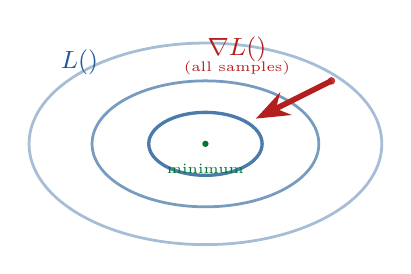
\begin{tikzpicture}[scale=0.8]
      % Define colors
      \definecolor{contourblue}{RGB}{30,90,150}
      \definecolor{gradred}{RGB}{180,30,30}
      \definecolor{pointred}{RGB}{200,50,50}
      \definecolor{minimumgreen}{RGB}{0,120,50}
      
      % Cleaner contours - fewer lines
      \draw[contourblue!40, line width=1pt] (0,0) ellipse (2.8 and 1.6);
      \draw[contourblue!60, line width=1pt] (0,0) ellipse (1.8 and 1);
      \draw[contourblue!80, line width=1.2pt] (0,0) ellipse (0.9 and 0.5);

      % Current point - simpler
      \coordinate (theta) at (2,1);
      \fill[pointred] (theta) circle (0.06);
      \node[pointred, font=\small] at (2.4,1.1) {$\vtheta$};

      % True gradient vector - smaller arrow
      \draw[-{Stealth[scale=1.0]}, gradred, line width=2pt] 
        (theta) -- +(-1.2,-0.6);
      
      % Clean labels
      \node[gradred, font=\small] at (0.5,1.5) {$\nabla L(\vtheta)$};
      \node[gradred, font=\tiny] at (0.5,1.2) {(all samples)};

      % Global minimum
      \fill[minimumgreen] (0,0) circle (0.05);
      \node[minimumgreen, font=\tiny] at (0,-0.4) {minimum};

      % Surface label
      \node[contourblue, font=\small] at (-2,1.3) {$L(\vtheta)$};
    \end{tikzpicture}
    \end{center}
    
    \vspace{0.5cm}
    \begin{keypointsbox}{}
    {\scriptsize Gradient uses ALL data points for true direction}
    \end{keypointsbox}
  \end{frame}

  \begin{frame}{Visual Intuition 2: Individual Sample Loss Surfaces}
    \textbf{Loss for individual data points (different shapes):}
    
    \begin{center}
    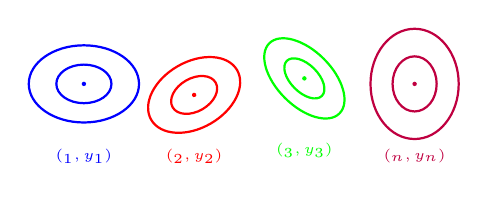
\begin{tikzpicture}[scale=0.7]
      % Individual loss surface 1 - more compact
      \begin{scope}[shift={(-3,0)}]
      \draw[blue, thick] (0,0) ellipse (1.0 and 0.7);
      \draw[blue, thick] (0,0) ellipse (0.5 and 0.35);
      \fill[blue] (0,0) circle (0.04);
      \node[blue, below] at (0,-1.0) {\tiny $(\vx_1, y_1)$};
      \end{scope}

      % Individual loss surface 2 
      \begin{scope}[shift={(-1,-0.2)}, rotate=30]
      \draw[red, thick] (0,0) ellipse (0.9 and 0.6);
      \draw[red, thick] (0,0) ellipse (0.45 and 0.3);
      \fill[red] (0,0) circle (0.04);
      \end{scope}
      \node[red, below] at (-1,-1.0) {\tiny $(\vx_2, y_2)$};

      % Individual loss surface 3
      \begin{scope}[shift={(1,0.1)}, rotate=-45]
      \draw[green, thick] (0,0) ellipse (0.9 and 0.5);
      \draw[green, thick] (0,0) ellipse (0.45 and 0.25);
      \fill[green] (0,0) circle (0.04);
      \end{scope}
      \node[green, below] at (1,-0.9) {\tiny $(\vx_3, y_3)$};

      % Sample n loss surface
      \begin{scope}[shift={(3,0)}]
      \draw[purple, thick] (0,0) ellipse (0.8 and 1.0);
      \draw[purple, thick] (0,0) ellipse (0.4 and 0.5);
      \fill[purple] (0,0) circle (0.04);
      \end{scope}
      \node[purple, below] at (3,-1.0) {\tiny $(\vx_n, y_n)$};
    \end{tikzpicture}
    \end{center}
    
    \pause
    \begin{alertbox}{Key Observation}
    {\small Each individual gradient points in a \textbf{different direction} - some variation!}
    \end{alertbox}
  \end{frame}

  \begin{frame}{Visual Intuition 3: Averaging Individual Gradients}
    \textbf{The magic: Average of individual gradients = True gradient}
    
    \begin{center}
    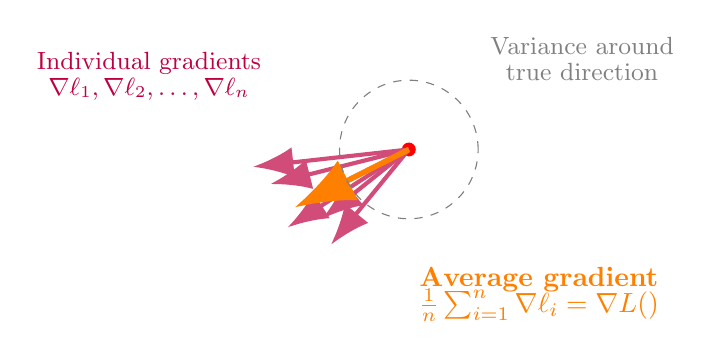
\begin{tikzpicture}[scale=1.1]
      % Current point
      \coordinate (theta) at (0,0);
      \fill[red] (theta) circle (0.08);
      \node[red] at (0,-0.4) {$\vtheta$};

      % Individual gradient vectors (purple, different directions)
      \draw[-{Latex[scale=1.5]}, purple!70, line width=1.5pt] (theta) -- +(-1.2,-0.6);
      \draw[-{Latex[scale=1.5]}, purple!70, line width=1.5pt] (theta) -- +(-1.8,-0.2);
      \draw[-{Latex[scale=1.5]}, purple!70, line width=1.5pt] (theta) -- +(-0.9,-1.1);
      \draw[-{Latex[scale=1.5]}, purple!70, line width=1.5pt] (theta) -- +(-1.4,-0.9);
      \draw[-{Latex[scale=1.5]}, purple!70, line width=1.5pt] (theta) -- +(-1.6,-0.4);
      \draw[-{Latex[scale=1.5]}, purple!70, line width=1.5pt] (theta) -- +(-1.0,-0.8);
      
      % Average gradient (reasonably thick but not overwhelming)
      \draw[-{Latex[scale=1.8]}, orange, line width=2pt] (theta) -- +(-1.32,-0.67);
      
      % Labels
      \node[purple] at (-3,1) {\small Individual gradients};
      \node[purple] at (-3,0.7) {\small $\nabla \ell_1, \nabla \ell_2, \ldots, \nabla \ell_n$};
      
      \node[orange] at (1.5,-1.5) {\textbf{Average gradient}};
      \node[orange] at (1.5,-1.8) {$\frac{1}{n}\sum_{i=1}^n \nabla \ell_i = \nabla L(\vtheta)$};

      % Show variance with dotted circle
      \draw[dashed, gray] (theta) circle (0.8);
      \node[gray] at (2,1.2) {\small Variance around};
      \node[gray] at (2,0.9) {\small true direction};
    \end{tikzpicture}
    \end{center}
    
    \begin{theorembox}{Visual Proof of Unbiasedness}
    {\small Even though individual gradients vary, their average equals the true gradient!}
    \end{theorembox}
  \end{frame}

  \begin{frame}{Visual Intuition 4: SGD Sampling Process}
    \textbf{SGD randomly picks one gradient at a time:}
    
    \begin{center}
    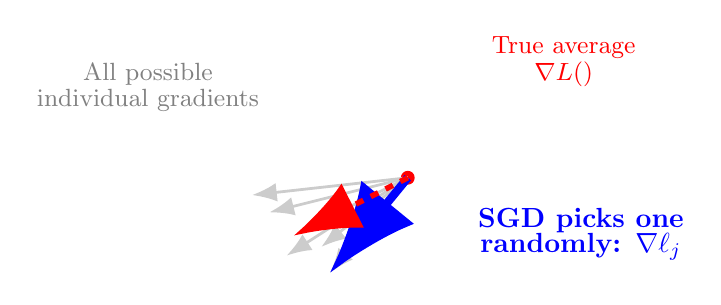
\begin{tikzpicture}[scale=1.1]
      % Current point
      \coordinate (theta) at (0,0);
      \fill[red] (theta) circle (0.08);
      \node[red] at (0,-0.4) {$\vtheta$};

      % Show all possible gradients (light gray)
      \draw[-{Latex[scale=1.2]}, gray!40, line width=1pt] (theta) -- +(-1.2,-0.6);
      \draw[-{Latex[scale=1.2]}, gray!40, line width=1pt] (theta) -- +(-1.8,-0.2);
      \draw[-{Latex[scale=1.2]}, gray!40, line width=1pt] (theta) -- +(-0.9,-1.1);
      \draw[-{Latex[scale=1.2]}, gray!40, line width=1pt] (theta) -- +(-1.4,-0.9);
      \draw[-{Latex[scale=1.2]}, gray!40, line width=1pt] (theta) -- +(-1.6,-0.4);
      \draw[-{Latex[scale=1.2]}, gray!40, line width=1pt] (theta) -- +(-1.0,-0.8);
      
      % Highlight one selected gradient (thick blue)
      \draw[-{Latex[scale=2]}, blue, line width=3pt] (theta) -- +(-0.9,-1.1);
      
      % True average (dashed red)
      \draw[-{Latex[scale=2]}, red, dashed, line width=2pt] (theta) -- +(-1.32,-0.67);
      
      % Labels
      \node[gray] at (-3,1.2) {\small All possible};
      \node[gray] at (-3,0.9) {\small individual gradients};
      
      \node[blue] at (2,-0.5) {\textbf{SGD picks one}};
      \node[blue] at (2,-0.8) {\textbf{randomly: $\nabla \ell_j$}};
      
      \node[red] at (1.8,1.5) {\small True average};
      \node[red] at (1.8,1.2) {\small $\nabla L(\vtheta)$};
    \end{tikzpicture}
    \end{center}
    
    \begin{keypointsbox}{}
    {\small \textbf{Key insight:} Sometimes SGD goes "wrong" direction, but on average it's correct!}
    \end{keypointsbox}
  \end{frame}

  \begin{frame}{Why Unbiasedness Matters in Practice}
    \pause
    \begin{examplebox}{Intuitive Analogy}
    Like asking random people for directions:
    \begin{itemize}
        \item Each person's answer might be slightly off
        \item But if there's no systematic bias, the average is correct
        \item SGD does the same with gradient estimates!
    \end{itemize}
    \end{examplebox}
  \end{frame}

  \section{Computational Complexity}

  \begin{frame}{GD vs Normal Equation: Complexity}
    \textbf{For linear regression:}
    
    \begin{alertbox}{Normal Equation}
    $\hat{\vtheta} = (\mX^T\mX)^{-1}\mX^T\vy$
    \\\textbf{Time:} $\mathcal{O}(d^2n + d^3)$
    \\\textbf{Space:} $\mathcal{O}(d^2)$ 
    \end{alertbox}
    
    \pause
    \begin{keypointsbox}{Gradient Descent}  
    $\vtheta_{t+1} = \vtheta_t - \alpha \mX^T(\mX\vtheta_t - \vy)$
    \\\textbf{Time:} $\mathcal{O}(T \cdot nd)$ for $T$ iterations
    \\\textbf{Space:} $\mathcal{O}(nd)$
    \end{keypointsbox}
  \end{frame}

  \begin{frame}{When to Use Which Method}
    \begin{keypointsbox}{}
    \textbf{Modern ML:} Gradient descent dominates due to:
    \begin{itemize}
        \item High-dimensional data ($d$ very large)
        \item Non-linear models (no normal equation exists)
        \item Large datasets ($n$ very large)
    \end{itemize}
    \end{keypointsbox}
    
    \pause
    \textbf{Decision criteria:}
    \begin{itemize}[<+->]
        \item \textbf{Few features ($d < 1000$):} Consider normal equation
        \item \textbf{Many features ($d > 10000$):} Gradient descent
        \item \textbf{Non-linear models:} Only gradient descent works
        \item \textbf{Online learning:} Only gradient descent works
    \end{itemize}
  \end{frame}

  \section{Advanced Topics and Extensions}

  \begin{frame}{Beyond Basic Gradient Descent}
    \textbf{Modern optimizers improve upon vanilla GD:}
    
    \begin{itemize}[<+->]
        \item \textbf{Momentum:} $\vv_{t+1} = \beta \vv_t + (1-\beta)\vg_t$
        \item \textbf{AdaGrad:} Adaptive per-parameter learning rates
        \item \textbf{Adam:} Combines momentum + adaptive rates  
        \item \textbf{RMSprop:} Exponential moving average of squared gradients
    \end{itemize}
    
    \pause
    \textbf{Why these improvements?}
    \begin{itemize}[<+->]
        \item Handle different parameter scales automatically
        \item Accelerate convergence in relevant directions
        \item Reduce oscillations in narrow valleys
    \end{itemize}
  \end{frame}

  \begin{frame}{Gradient Descent in Deep Learning}
    \begin{keypointsbox}{}
    Every deep learning framework uses gradient descent variants!
    \end{keypointsbox}
    
    \pause
    \textbf{Key modern extensions:}
    \begin{itemize}[<+->]
        \item \textbf{Backpropagation:} Efficient gradient computation
        \item \textbf{Automatic differentiation:} PyTorch/TensorFlow magic
        \item \textbf{GPU acceleration:} Parallel mini-batch processing
        \item \textbf{Mixed precision:} 16-bit + 32-bit arithmetic
    \end{itemize}
  \end{frame}

  \section{Practical Considerations}

  \begin{frame}{Learning Rate Selection Strategies}
    \textbf{Common approaches:}
    
    \begin{itemize}[<+->]
        \item \textbf{Grid search:} Try $\{0.001, 0.01, 0.1, 1.0\}$
        \item \textbf{Learning rate schedules:} Start high, decay over time
        \item \textbf{Adaptive methods:} Let algorithm adjust automatically  
        \item \textbf{Learning rate finder:} Gradually increase and monitor
    \end{itemize}
    
    \pause
    \textbf{Warning signs:}
    \begin{itemize}[<+->]
        \item Loss exploding $\rightarrow$ $\alpha$ too high
        \item Very slow progress $\rightarrow$ $\alpha$ too low
        \item Oscillating loss $\rightarrow$ Try momentum or smaller $\alpha$
    \end{itemize}
  \end{frame}

  \begin{frame}{Convergence Criteria}
    \textbf{When to stop training?}
    
    \begin{itemize}[<+->]
        \item \textbf{Gradient magnitude:} $||\nabla f(\vtheta)|| < \epsilon$
        \item \textbf{Function change:} $|f(\vtheta_{t+1}) - f(\vtheta_t)| < \epsilon$
        \item \textbf{Parameter change:} $||\vtheta_{t+1} - \vtheta_t|| < \epsilon$
        \item \textbf{Maximum iterations:} Always set an upper bound
    \end{itemize}
    
    \pause
    \begin{keypointsbox}{}
    \textbf{Best practice:} Use multiple criteria + validation performance
    \end{keypointsbox}
  \end{frame}

  \begin{frame}{Common Pitfalls}
    \begin{alertbox}{Pitfall 1: Poor Initialization}
    \textbf{Problem:} Bad starting points
    \\\textbf{Solution:} Xavier/He initialization
    \end{alertbox}
    
    \pause
    \begin{alertbox}{Pitfall 2: Wrong Learning Rate}
    \textbf{Problem:} Divergence or slow convergence
    \\\textbf{Solution:} Learning rate schedules, adaptive optimizers
    \end{alertbox}
    
    \pause
    \begin{alertbox}{Pitfall 3: Poor Feature Scaling}
    \textbf{Problem:} Different scales cause poor convergence
    \\\textbf{Solution:} Standardize features: $(x - \mu)/\sigma$
    \end{alertbox}
  \end{frame}

  \section{Summary and Key Takeaways}

  \begin{frame}{What We've Learned}
    \begin{keypointsbox}{}
    Gradient descent is the backbone of modern machine learning!
    \end{keypointsbox}
    
    \pause
    \textbf{Journey recap:}
    \begin{itemize}[<+->]
        \item \textbf{Mathematical foundation:} Taylor series derivation
        \item \textbf{Geometric intuition:} Steepest descent direction
        \item \textbf{Algorithm variants:} Batch, SGD, mini-batch
        \item \textbf{Theoretical properties:} Unbiased estimator guarantees
        \item \textbf{Practical wisdom:} Learning rates, scaling, diagnostics
    \end{itemize}
  \end{frame}

  \begin{frame}{From Theory to Practice}
    \textbf{Next steps for mastery:}
    \begin{itemize}[<+->]
        \item Implement gradient descent from scratch
        \item Experiment with different learning rates
        \item Compare batch vs SGD vs mini-batch
        \item Try advanced optimizers (Adam, momentum)
        \item Apply to real datasets
    \end{itemize}
    
    \pause
    \begin{keypointsbox}{}
    Master gradient descent first - it's the foundation for everything else!
    \end{keypointsbox}
  \end{frame}

  \stepcounter{popquiz}
  \begin{frame}{Final Pop Quiz \#\thepopquiz}
    \begin{popquizbox}{\thepopquiz}
    \textbf{True or False?}
    \begin{enumerate}
        \item SGD always converges faster than batch GD
        \item Learning rates should decrease during training  
        \item SGD gradient estimates are unbiased
        \item Normal equation always beats gradient descent
        \item GD guarantees global minimum for any function
    \end{enumerate}
    \end{popquizbox}
  \end{frame}

  % Include SGD theory deep dive
  \begin{frame}{Deep Dive: Advanced Theory}
    \begin{center}
    \textbf{For comprehensive mathematical analysis:}
    \end{center}
    
    \begin{alertbox}{Reference Materials}
    \begin{itemize}
        \item SGD.pdf: Detailed convergence proofs  
        \item Florian's estimators: \url{https://florian.github.io/estimators/}
        \item Interactive notebooks for hands-on practice
    \end{itemize}
    \end{alertbox}
  \end{frame}

  % SGD.pdf reference - see assets folder for detailed theory

  % Quiz solutions
  \begin{frame}{Pop Quiz Solutions}
    \textbf{Quiz \#1 Solutions:} 
    \begin{enumerate}
        \item $f(2) = 6$, $f^{\prime}(2) = 4$
        \item $f(x) \approx 6 + 4(x-2)$
        \item New $x = 2 - 0.1 \times 4 = 1.6$
        \item Yes, function decreases!
    \end{enumerate}
    
    \pause
    \textbf{Quiz \#2 Solutions:}
    \begin{enumerate}
        \item False - SGD faster per epoch, may need more epochs
        \item True - schedules often improve convergence
        \item True - key theoretical property  
        \item False - only for linear problems, small $d$
        \item False - only local minima; global for convex only
    \end{enumerate}
  \end{frame}

  \begin{frame}
    \centering
    \Huge \textbf{Thank You!}
    
    \vspace{1cm}
    \Large Questions?
    
    \vspace{1cm}
    \normalsize
    \textbf{Next:} Advanced Optimization Techniques
    
    \textbf{Practice:} Implement GD for your favorite ML model!
  \end{frame}

\end{document}